\section{Market Microstructure}

Market microstructure is the study of the trading mechanics that are in place 
in real markets. It describes why trading occurs, the rules of trading 
and the protocols to form a trade. \citep[p. 3-4]{Has07}
Understanding market microstructure is cruicial in designing an artificial market
as without realistic trading settings the representativeness of the model may end
up to be poor and have limited practicality. The goal of an artificial market often
is to recreate phenomena from the real world in a well understood and controlled 
environment thus the link to the real world should be maintained. In addition to the
common properties that the existing markets often share and the general distinctions between
types of markets that exist,
 the common observed price phenomena is discussed. These price phenomena, called
stylished facts, are often used in validating the artificial models.

% TODO: Maybe extend with behavioural aspects?

\subsection{Double Auction}
% Call-market (Itayose, Sealed-bid) vs CDA (Zaraba)

Financial markets are most often organized as double auction markets.
Double auction market (DA) is a special type of auction in which there
are multiple buyers and sellers which are both able to 
produce quotes and they are treated symmetrically \citep*{Kle99}. Buyers
make offers to buy, bid, the traded asset while sellers make offers
to sell, ask, the traded asset \citep*{Moc15}. There are some variations 
between double auction markets. They generally differ in when the clearing process takes place 
and how the orders are matched. 
%In some implementations, such as 
%\citet*{God93}'s, a trade is formed only when a buyer and a seller 
%each agree on the exact trade price but typically the matching of crossing orders is automated.

% \subsubsection{Order Matching in Double Auction}

Main distinction between double auction market models is when
the order matching takes place. Typically, the order matching 
is continuous process occuring after the arrival of each new order but
in some markets this process takes place after a specified time interval
has passed, for example at the end of a trading day. \citep{boer05}
In auction literature, there are various terms used to describe essentially 
the same mechanics. \citet{boer05} used term 
\textit{continuous session market} for the former and \textit{call-market}
for the latter whereas \citet{ASt05} called them \textit{Itayose method}
and \textit{Zaraba method} respectively. \citet{Moc15} used term \textit{continuous 
double auction} (CDA) for the former and \textit{periodic double auction} to describe 
the same mechanics of call-markets as which they described is an extension of 
a type of auction called sealed-bid. In sealed-bid auctions the bid and ask offers
are submitted once and then the order matching is executed once. In this thesis
the terms continuous double auction and call-markets are chosen to describe
these types of markets as they seem to be the most prevalent in the literature.

In call-market the orders are cumulated for a specified period of time and the
market is cleared with a single price whereas in continuous market it is done
whenever there are orders that can be matched and the price is derived from these
orders. \citep{boer05} 
Many real world stock markets are formed as a hybrid of call and continuous
double auction markets. The price discovery at the beginning and at the end of a 
trading day is conducted with call-market mechanics and the trading during the 
typical trading hours is conducted using continuous environment. \citet{NasdaqClosing05}
For example, Nasdaq's opening and closing call-auctions, called opening and closing crosses,
create the official open and close prices of the market \citet{NasdaqCrosses}.  
% More about Sealed-bid matching (supply-demand) and CDA matching
 
\subsection{Execution Systems}
% Quote-driven vs Order-driven
The execution systems are typically divided into two types:
quote-driven and order-driven execution systems. In quote-driven market, also known
as intermediate markets, the investors trade with prices provided 
by dealers or intermediaries who are part of the market organization. 
In order-driven market, also called as limit order market, 
the prices are formed according to the orders submitted by the 
investors themselves and trades are formed in a centralized marketplace 
via automatic order matching or with the help of market makers. 
\citep{Baru17} According to \citet{MALINOVA2013104},
the liquidity and price efficiency are generally higher in order-driven 
markets. They also found out that smaller orders get more favorable prices in 
quote-driven markets due to smaller bid-ask spread 
but larger orders benefit from order-driven markets because of the lower 
execution costs. Quote-driven markets are also less transparent compared
to order-driven markets. Real markets, however, are most often a combination
of the two \citep{boer05} but recently there have been a trend to move from quote-driven
markets to order-driven markets \citep{MALINOVA2013104}.

As simulating intermediate market participants increases compexity
of the model, artificial markets with realistic quote-driven execution are rare. 
However, some artificial markets, such as \citet{SantaFe99}'s, do have some of 
the elements of quote-driven markets in a sense that the prices are driven by 
the sizes of the orders and not prices offered by the investors or traders. 
Most of the artificial markets found in the ASM literature seem to be order-driven.
% Challenges of quote-driven (clearing is non trivial)

\subsection{Price Formation}
% Order book, matching and clearing
% Why we don't go deeper to quote-driven:
Price formation is direct product of the execution system in place in a market
\citep{boer05}. In order-driven markets it is direct result of the orders
in the market and the matching algorithm in place whereas in quote-driven markets it
is dependent on how the intermediaries view the current and future 
balance between supply and demand of the traded asset. The equilibrium price of a 
quote-driven market is driven by the orders sizes and in order-driven markets
it is driven by also the prices submitted with the orders. \citep{MALINOVA2013104}
As quote-driven markets' price formation is somewhat a black box due to the 
dependency on the views and intentions of the intermediaries, it was not considered
as the execution system for the model built in this thesis. On the other hand, 
the price formation of an order-driven market is dependent only on the orders in the
market and the predefined supply-demand matching algorithm in place thus its price 
formation can be described with greater level of generalization.

% Limit order book and terms
Limit order book is a core component in the price formation in order-driven markets.
Limit order book stores the submitted limit orders which are simply orders that contain the quantity and 
the limit price stated by the trader. Limit price is the maximum price, in case of bid, or the minimum
price, in case of ask, that the order is allowed to be cleared with. In other words,
bids (asks) cannot be cleared with a price higher (lower) than the limit price stated 
in the order. There are also other types of orders, such as market and 
stop-loss orders, but these can be seen as derivatives from limit orders: 
for example, a bid (an ask) market order is essentially a limit order 
with an extremely high (low) limit price so that it does get matched 
during the clearing process as long as there are opposing limit orders in the 
order book. \citep{lob13} %TODO: What if only market orders?


\begin{table}
\centering
\caption{A simple representation of order book}
\label{tbl:orderbook}
\begin{tabular}{lrr}
\toprule
{} &  Bid quantities &  Ask quantities \\
price &                 &                 \\
\midrule
5.04  &               0 &             600 \\
5.03  &               0 &             500 \\
5.02  &              50 &             600 \\
5.01  &             100 &             200 \\
5.00  &             100 &             200 \\
4.99  &             250 &             150 \\
4.98  &             400 &             150 \\
4.97  &             400 &             100 \\
4.96  &             700 &               0 \\
4.95  &             500 &               0 \\
\bottomrule
\end{tabular}
\end{table}
% table.tex > \mytable

% Basics of limit order book, supply and demand etc.
A simple limit order book is presented in ~\ref{tbl:orderbook}. This table shows the
quantity of asset bid and asked per each price level: for example, with a price of 5.00
there are 100 unit bid and 200 unit asked. There are, however, more bids and asks that 
accept this price. Those traders that have bid 5.01 and those that have asked 4.99 would obviously also accept
this price. Therefore it is more informatic to calculate cumulative sum of bid and reverse cumulative sum of 
ask quantities and come up with total quantities of bid and ask per price level that can be matched.  
This order book with cumulative quantities is visualized in figure ~\ref{fig:lob_visual}. Cumulative bids
are renamed as demand and cumulative asks as supply as these terms are more representative in this context.
As there should not be clearable orders in continuous double auction's order book, except very temporarily, 
this example represents more of the state of a limit order book in a call-market. Order book
in continuous double auction is discussed in a moment.

\begin{figure}
    \begin{center}  
        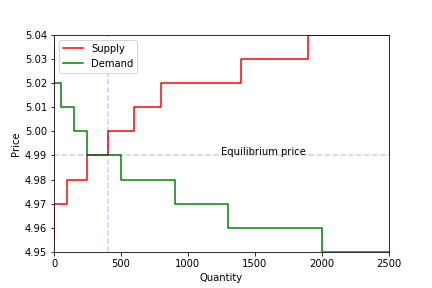
\includegraphics{plots/orderbook_visualized.png}
        \caption{Visualized order book}
        \label{fig:lob_visual}
    \end{center}
\end{figure}

% Price formation in sealed bid/call market
Call-markets typically clear at equilibrium price: at the point where
supply and demand crosses. 
To get the equlibrium price, first the maximum clearable quantity
is calculated per price level. This quantity is simply the element-wise
minimum from the supply and the demand arrays. Then the equilibrium volume
can be determined by taking the maximum from the maximum clearable quantities
per price level and equilibrium price is simply the price where the quantity
equals the equilibrium volume. A pseudocode of this algorithm is illustrated in 
algorithm ~\ref{alg:lob_equil}.

\begin{algorithm}[H]
    \SetAlgoLined
    \DontPrintSemicolon
    
    bids = sort\_ascending(bids, by price)\;
    asks = sort\_descending(asks, by price)\;
    \;
    demand = cumulative\_sum(bids, from quantity)\;
    supply = cumulative\_sum(asks, from quantity)\;
    \;
    maximum clearable per price = min\_quantity\_per\_price(demand, supply)\;
    \;
    equilibrium quantity = max(maximum clearable per price)\;
    equilibrium price = price where quantity is equilibrium quantity\;
    \KwResult{Equilibrium price and quantity}
    \caption{Pseudo algorithm for finding market equilibrium}
    \label{alg:lob_equil}
\end{algorithm}


In a continuous double auction, the matching process is slightly simpler in computation
wise as there is no need to find a common price for many orders. Only the latest arrived
order needs to be cleared, in case it can be cleared, with opposing orders. Continuous
double auction does not accumulate crossing orders in similar fashion as call markets do. 
In principle, the same algorithm used in call market could be used also in continuous double auction 
but typically the surplus distribution is different. Unlike in call-markets where the surplus is often
split, in continuous double auction the surplus goes to the trader who made the latest order.
In other words, the trade prices are taken from the orders that were already in the limit order book.
This sort of matching could be conducted by looping and clearing the opposing side of the order book until either
there are no more crossing orders with the newly arrived order or the new order is already cleared
completely. In case the newly arrived order is not completely cleared after depleting all the crossing
orders, it is inserted to the order book and the clearing process ends. This algorithm is illustrated in
algorithm ~\ref{alg:lob_cont}. 

\begin{algorithm}[H]
    \SetAlgoLined
    \DontPrintSemicolon
    \uIf{new order is bid}{
        asks = get\_asks(order book)\;
        price of new order = get\_price(new order)\;

        \While{(min\_price(asks) $\geq$ price of new order) \\
        \hskip\algorithmicindent\& (get\_quantity(new order) > 0)}{
            countering = filter(asks, where price $\geq$ get\_price(new order))\;
            opposite order = get\_next(countering)\;
            clear(new order, opposite order)\;
        }
    }
    \uElseIf{new order is ask}{
        bids = get\_bids(order book)\;
        price of new order = get\_price(new order)\;
        
        \While{(min\_price(bids) $\leq$ price of new order) \\ 
        \hskip\algorithmicindent \& (get\_quantity(new order) > 0)}{
            countering = filter(bids, where price $\leq$ get\_price(new order))\;
            opposite order = get\_next(countering)\;
            clear(new order, opposite order)\;
        }
    }
    \uIf{get\_quantity(new order) > 0}{
        insert\_to\_orderbook(new order)\;
    }

    \caption{Pseudo algorithm for clearing continuous double auction}
    \label{alg:lob_cont}
\end{algorithm}



\subsection{Price Dynamics}
% Stylized facts
The price dynamics in stock markets are known to be chaotic and difficult to 
analyze. The underlying elements that play a role in the price dynamics
are constantly evolving and it still remains relatively poorly understood.
However, there are some characteristics of price behaviour that are supported
with enough empirical evidence to be considered as properties of price in
financial markets. These statistical phenomena, called stylized facts in
econometrics, have been observed in extensive amount of studies from 
different assets, markets and time periods \citep{Shakeel18}. 
% List of Stylized facts (Cont R. (2001) & Gould et al. (2013))
The price related stylized facts are according to \citet{StylizedFacts01} and \citet{lob13}:

\begin{enumerate}
    \item Fat-tailed distribution of returns: distribution of asset returns have fatter tails than normal distribution meaning that they have positive excess kurtosis. 
    \par
    \begin{minipage}{\linewidth}
        \centering
        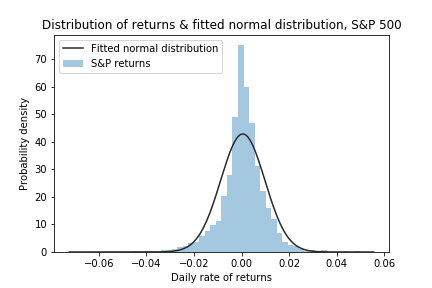
\includegraphics[width=10cm]{plots/S&P500_fat_tails.png}
        \captionof{figure}{Fat-tailed of returns of S\&P 500}
    \end{minipage}

    \item Lack of autocorrelation: autocorrelation of returns in financial markets have shown to be statistically insignificant, except in very short term. Previous returns have no prediction power over the future returns of a stock. 
    \par
    \begin{minipage}{\linewidth}
        \centering
        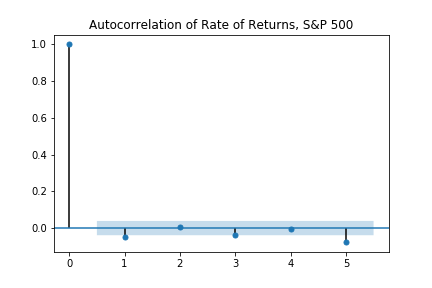
\includegraphics[width=10cm]{plots/S&P500_autocorr.png}
        \captionof{figure}{Absence of autocorrelation in S\&P 500}
    \end{minipage}

    \item Volatility clusters: volatility have measured to have positive autocorrelation. Big price movement tend to follow additional exceptional price movements forming clusters of volatility thorough time.
    \par
    \begin{minipage}{\linewidth}
        \centering
        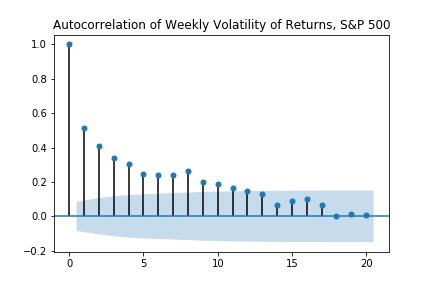
\includegraphics[width=10cm]{plots/S&P500_vola_autocorr.png}
        \captionof{figure}{Volatility clustering in S\&P 500}
    \end{minipage}
\end{enumerate} 

% Something about theories of these things (explanation for the stylized facts)
% file:///D:/Opinnot/Master's%20Thesis/literature/real%20markets/price%20dynamics/TheoriesExplainingStockPriceBehavior%20(1).pdf

As has been done in the literature of artificial markets, the 
representativeness of the ASM built in this thesis is validated also 
using these stylized facts.